\documentclass[]{article}
\usepackage{graphicx}

%opening
\title{Maximum entropy and population heterogeneity in continuous cell cultures meet experimental data, preliminary results}
\author{}

\begin{document}

\maketitle

%\begin{abstract}

%\end{abstract}


%\section{Introduction}



\section{Materials and Method} %%%%%%%%%%%%%%%%%%%%%%%%%%%%%%%%%%%%%%%%%%
%%%%%%%%%%%%%%%%%%%%%%%%%%%%%%%%%%%%%%%%%%%%%%%%%%%%%%%%%%%%%

\subsection{Experimental data} %%%%%%%%%%%%%%%%%%%%%%%%%%%%%%%%%%%%%%%%%%
	  
	Experimental data was taken from $Rath$, in this work the author performed 6 continuous cultures, ($A$, $B$, $C$, $D$, $E$, $F$), with the cell line AGE1.HN.AA1, which parental line AGE1.HN was established by the company ProBioGen (ProBioGen AG, Berlin, Germany) from a tissue sample of a human brain. All cultures feed mediums was based on the standard 42-Max-UB-medium, which is serum-free and was especially developed for the AGE1.HN cell line $Table 1$. The experiments was run under various conditions, differing mainly in the dilution rate ($D$) and the feed medium composition of glucose ($GLC$), glutamine ($GLN$) and galactose ($GAL$) $Table 2$. \\
	For each experiment, a steady state condition was reached, ($A$, $B$, $C$, $D$, $E$, $F01$), and several observables  was reported $Tables 3-4$. Particularly relevant for this work was the growth rate ($\mu$), $D$, the viable cell density ($Xv$) and the medium concentration ($s$) and derived uptake rate ($u$) for a set of metabolites ($GLC$, lactose ($LAC$), $GLN$, ammonium ($NH4$), $GAL$, pyruvate ($PYR$), glutamate ($GLU$), alanine ($ALA$), asparagine ($ASP$)). Unit conversion was required for make experimental data and models compatible. For this propose the only external data needed was the cell mass density. It was used  0.25 pgDW/ $\mu$$m^3$ $Niklas$.
	 
	 \begin{table}
	 	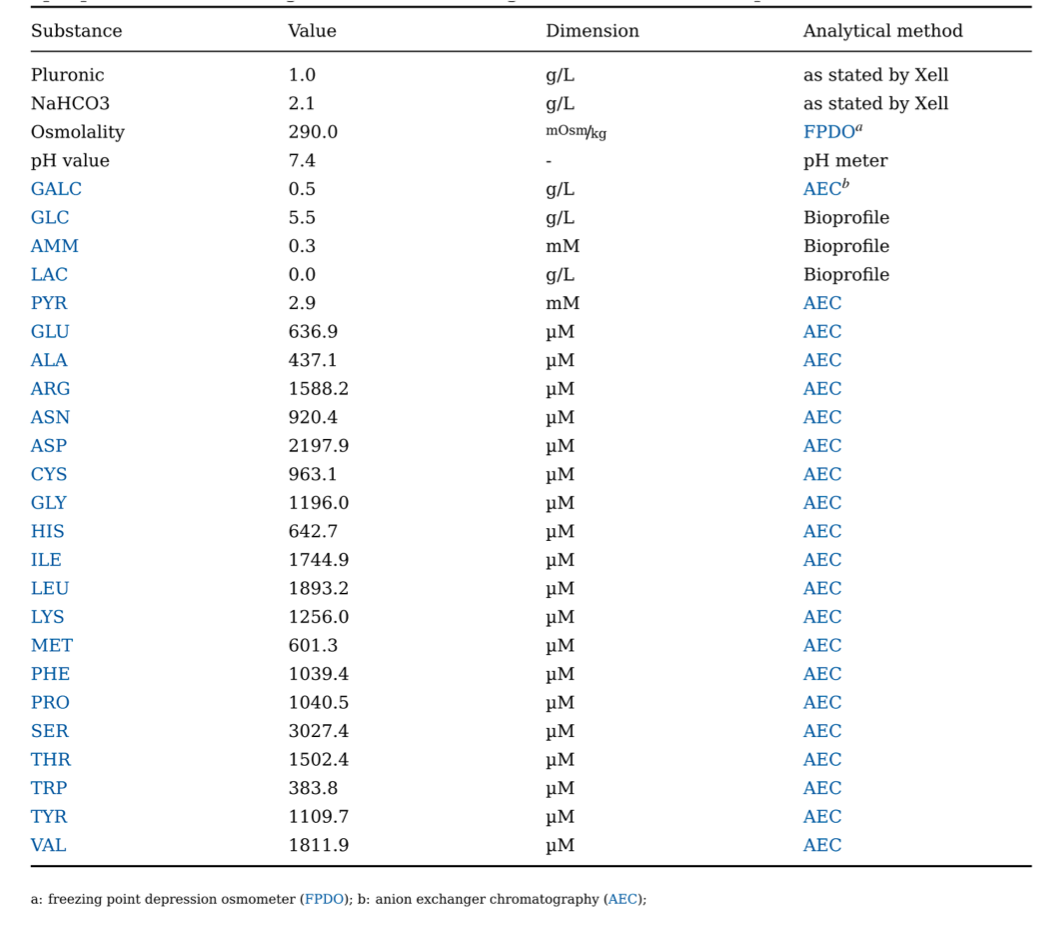
\includegraphics[scale = 0.7]{Table_3_1}
	 	\caption{Measured medium composition of the 42-MAX-UB standard medium. Extracted from $Rath$}
	 	
	 \end{table}
	 
	 \begin{table}
	 	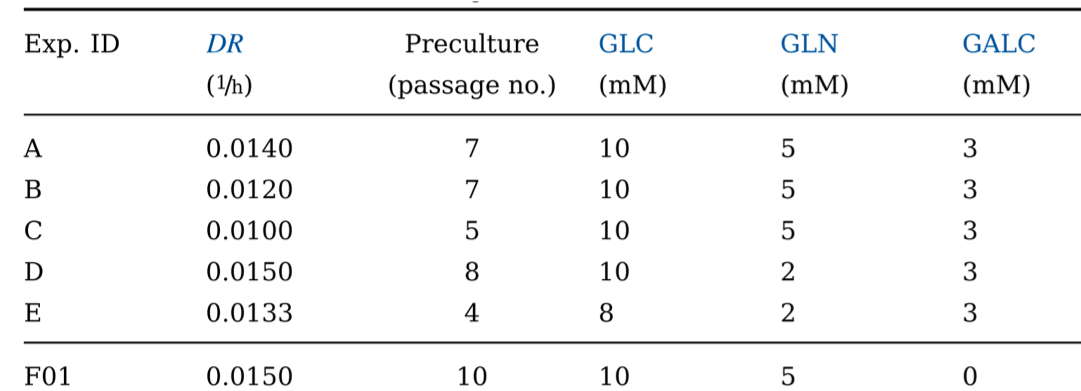
\includegraphics[scale = 0.7]{Table_4_10}
	 	\caption{The dilution rates, preculture ages and the 42-Max-UB-medium modified components concentrations used in $Rath$ for the 6 steady states. Table adapted from $Rath$}
	 	
	 \end{table}

	\begin{table}
		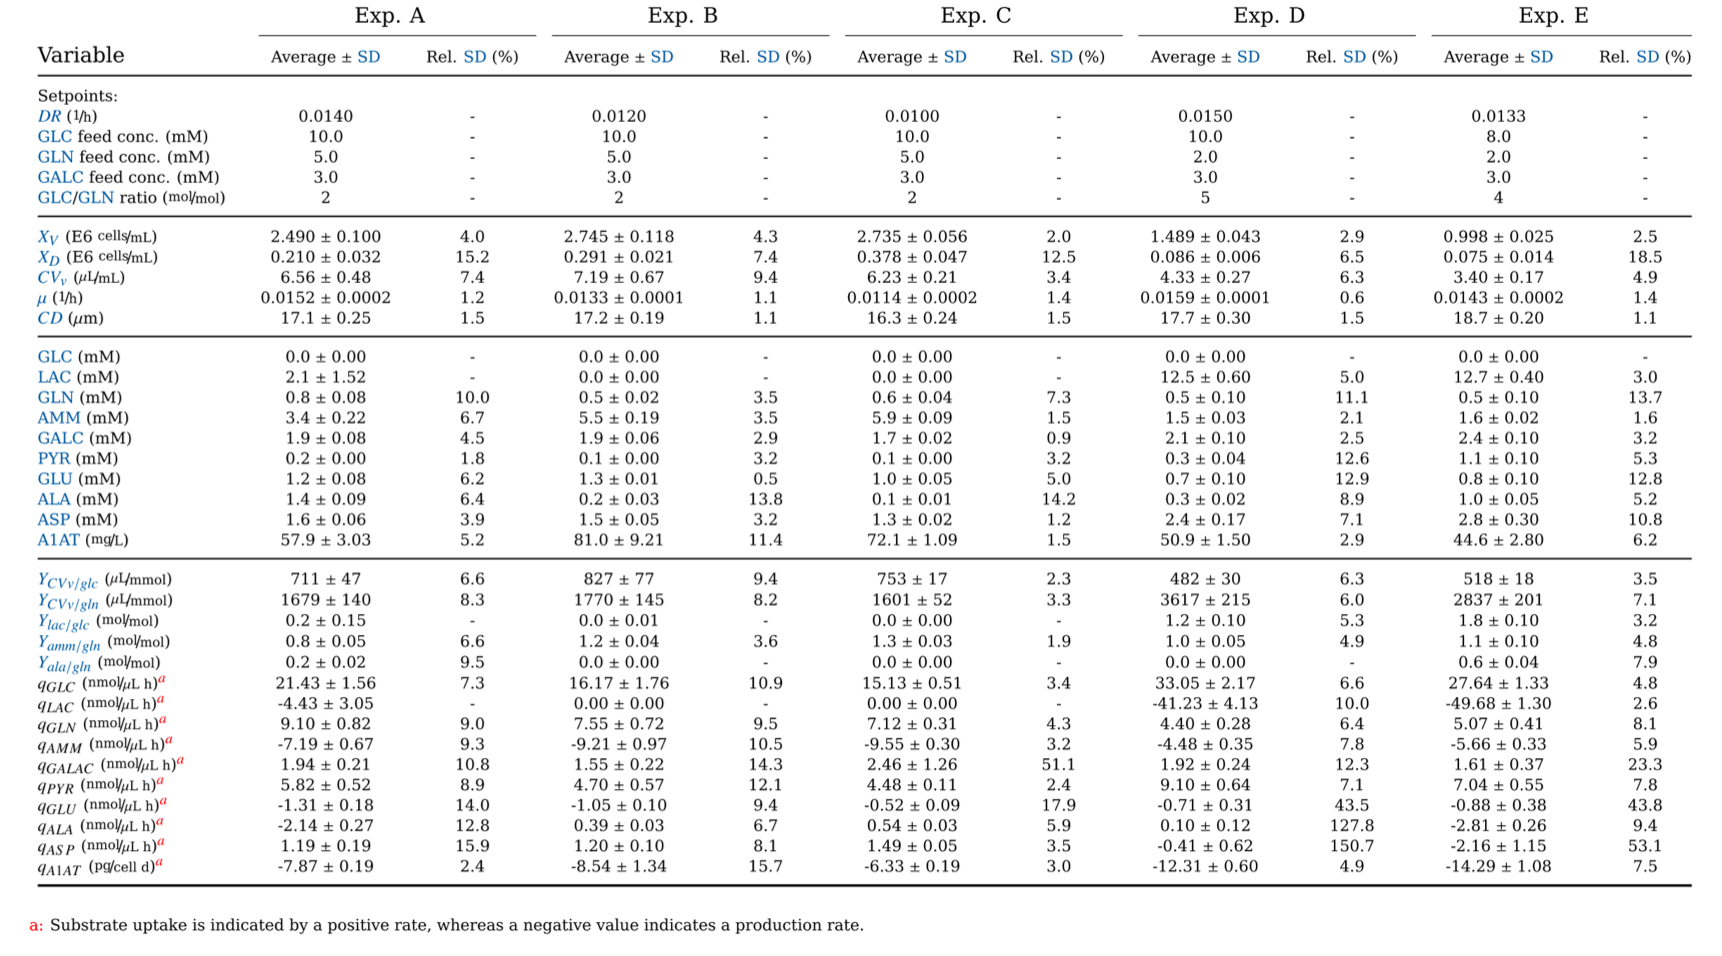
\includegraphics[scale = 0.7]{Table_4_11}
		\caption{The dilution rates, preculture ages and the 42-Max-UB-medium modified components concentrations used in $Rath$ for the 6 steady states. Table adapted from $Rath$}
		
	\end{table}

\subsection{Preparing GEMs} %%%%%%%%%%%%%%%%%%%%%%%%%%%%%%%%%%%%%%%%%%%
	
	In order to evaluate the capacity of the ...
	
	\subsubsection{Recon3d}

	Recon3DModel\_301.mat was downloaded from http://vmh.life [2], the biomass equation was modified to adjust the biomass demand reported by [1] for the cell line AGE1\_HN. All the others original demands from recon3d were deactivated. An extra demand representing the maintenance demand of atp was set according to [5]. All the fluxes representing exchangeable metabolites (external reactions) were set as reversible (lb and ub set to a big number), so the only effective constraints (for FBA and EP) is the one produced by the chemostat consideration[4]. Additionally, to include the molecular crowding constraints we map [7] enzymatic costs, initially defined for recon1, to recon3d.\\
	The external metabolites concentrations was set according 42\_MAX\_UB feed medium [6] for each of the 6 continuous cultivation conditions. A set of extra external metabolites, not specified in the medium, was also added. Particularly, Recon3d was unable to growth without pe\_hs[e], Phosphatidylethanolamine,  (or similar) lipid in the feeding medium. Later we will discuss the impact of this metabolite in the medium.
	
	\subsubsection{CHO}
	
	CHO bla bla... buscar como Cossio setea CHO en primer lugar.  The external metabolites concentrations was set similar to Recon3d for each experiment. The only different was that CHO is able to growth without pe\_hs[e], named pe\_cho\_e. 
	


\section{Results} %%%%%%%%%%%%%%%%%%%%%%%%%%%%%%%%%%%%%%%%%%%%%%%%%%
%%%%%%%%%%%%%%%%%%%%%%%%%%%%%%%%%%%%%%%%%%%%%%%%%%%%%%%%%%%%

\subsection{Low concentrations of phosphatidylethanolamine} %%%%%%%%%%%%%%%%%%%%%%%

		Here are shown the results for the experiments with 0.1 mM for Recon3D and 0 mM for CHO of phosphatidylethanolamine in the feed medium.
		
	\begin{figure}[h]
		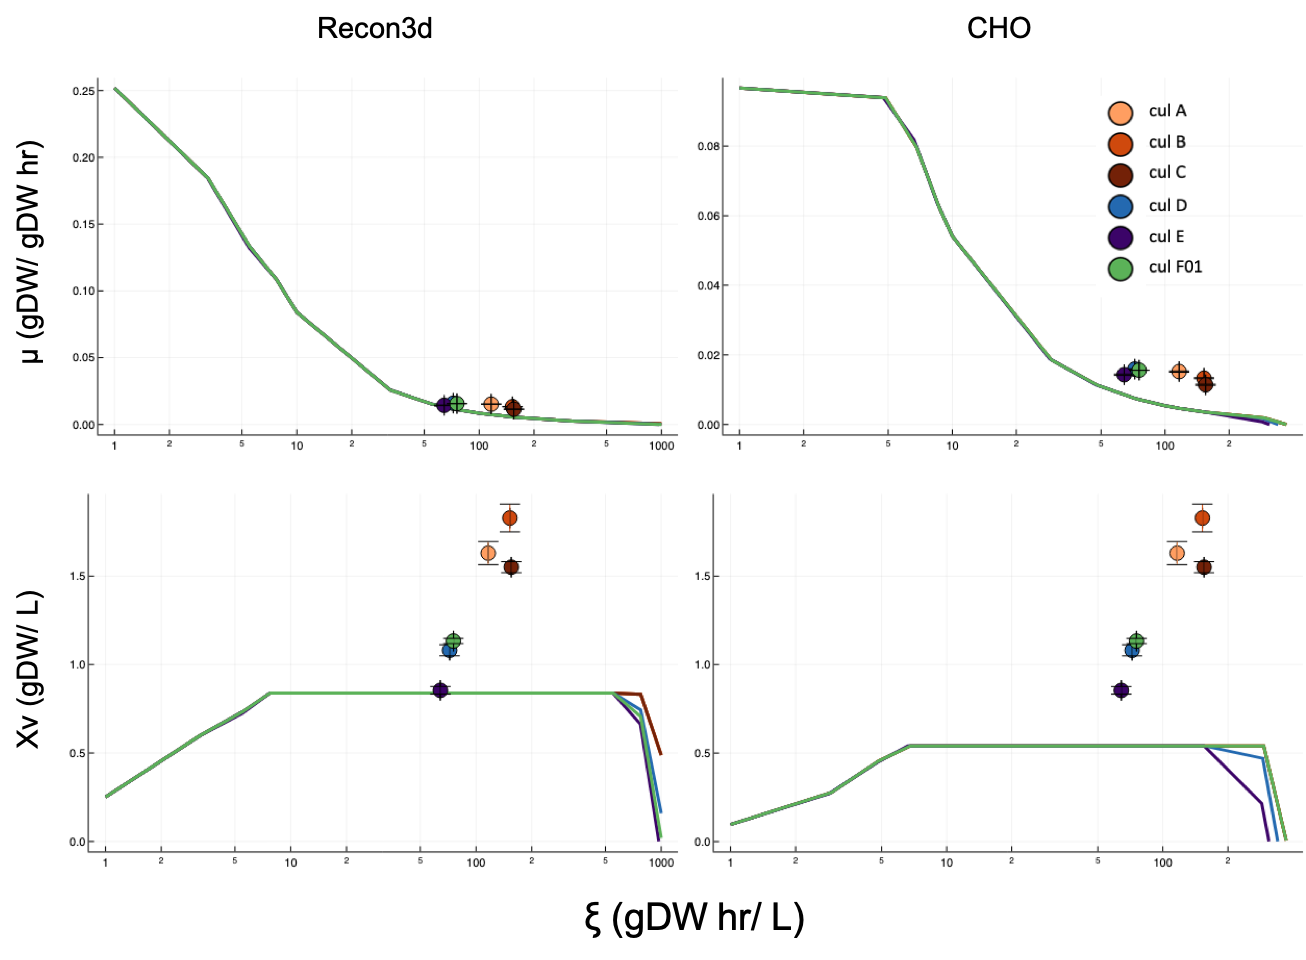
\includegraphics[scale = 0.5]{low_medium_1}
		\caption{FBA results showing the growth rate and the viable cell density dependence of $\xi$ for the six culture conditions. The solid lines represents the model predictions and the color points shows the experimental results. The data was obtained for feed mediums with low concentrations of phosphatidylethanolamine}
		
	\end{figure}
	
	\begin{figure}[!h]
		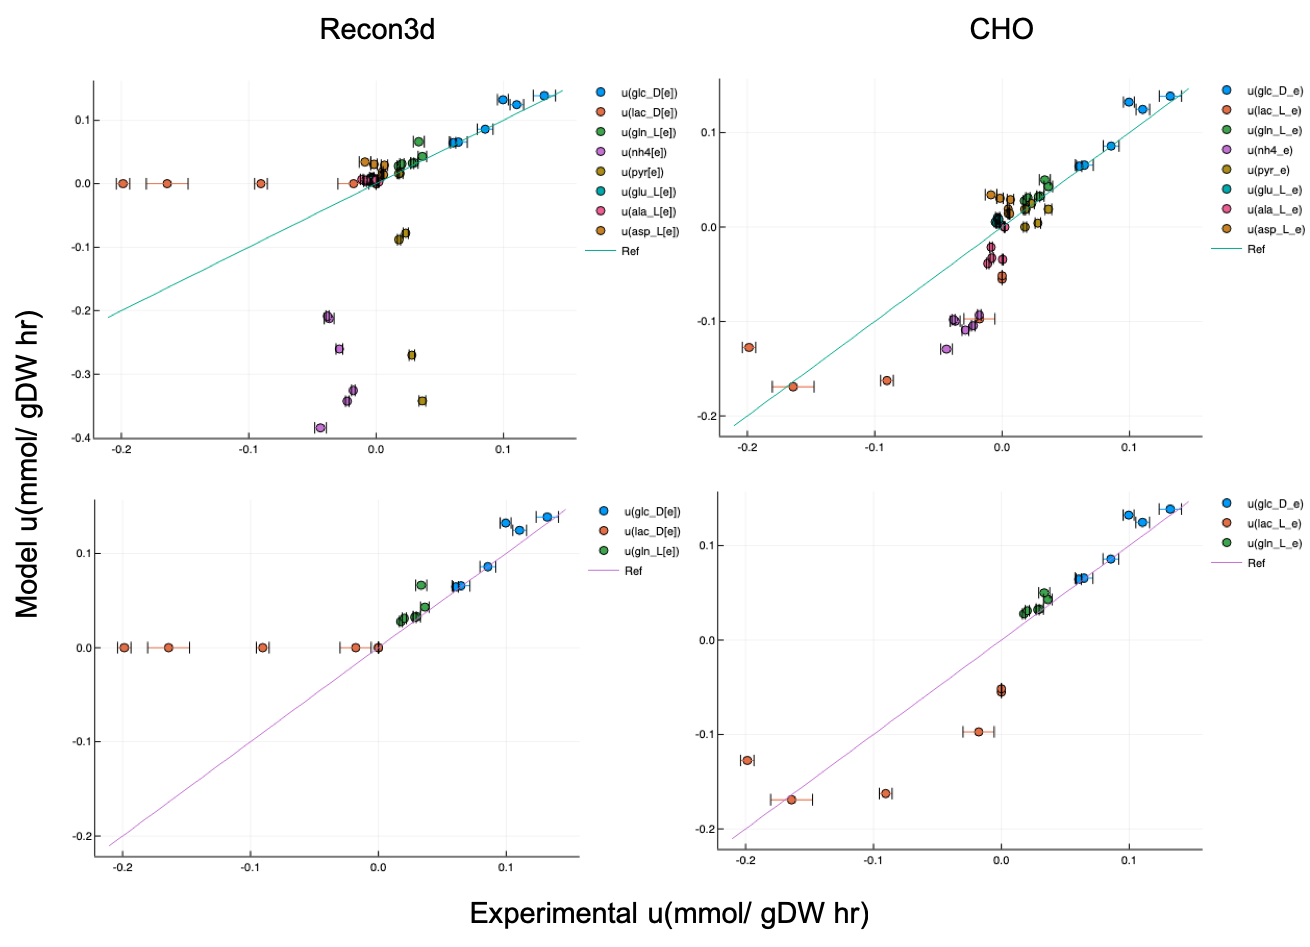
\includegraphics[scale = 0.5]{low_medium_2}
		\caption{Correlations of all the experimental uptakes, upper graphs, and a selected subset, inferior graphs, respect to the predicted value from for the experiments with low concentration of phosphatidylethanolamine.}
		
	\end{figure}

	\subsection{High concentrations of phosphatidylethanolamine} %%%%%%%%%%%%%%%%%%%%%%%
		
	\begin{figure}[h]
		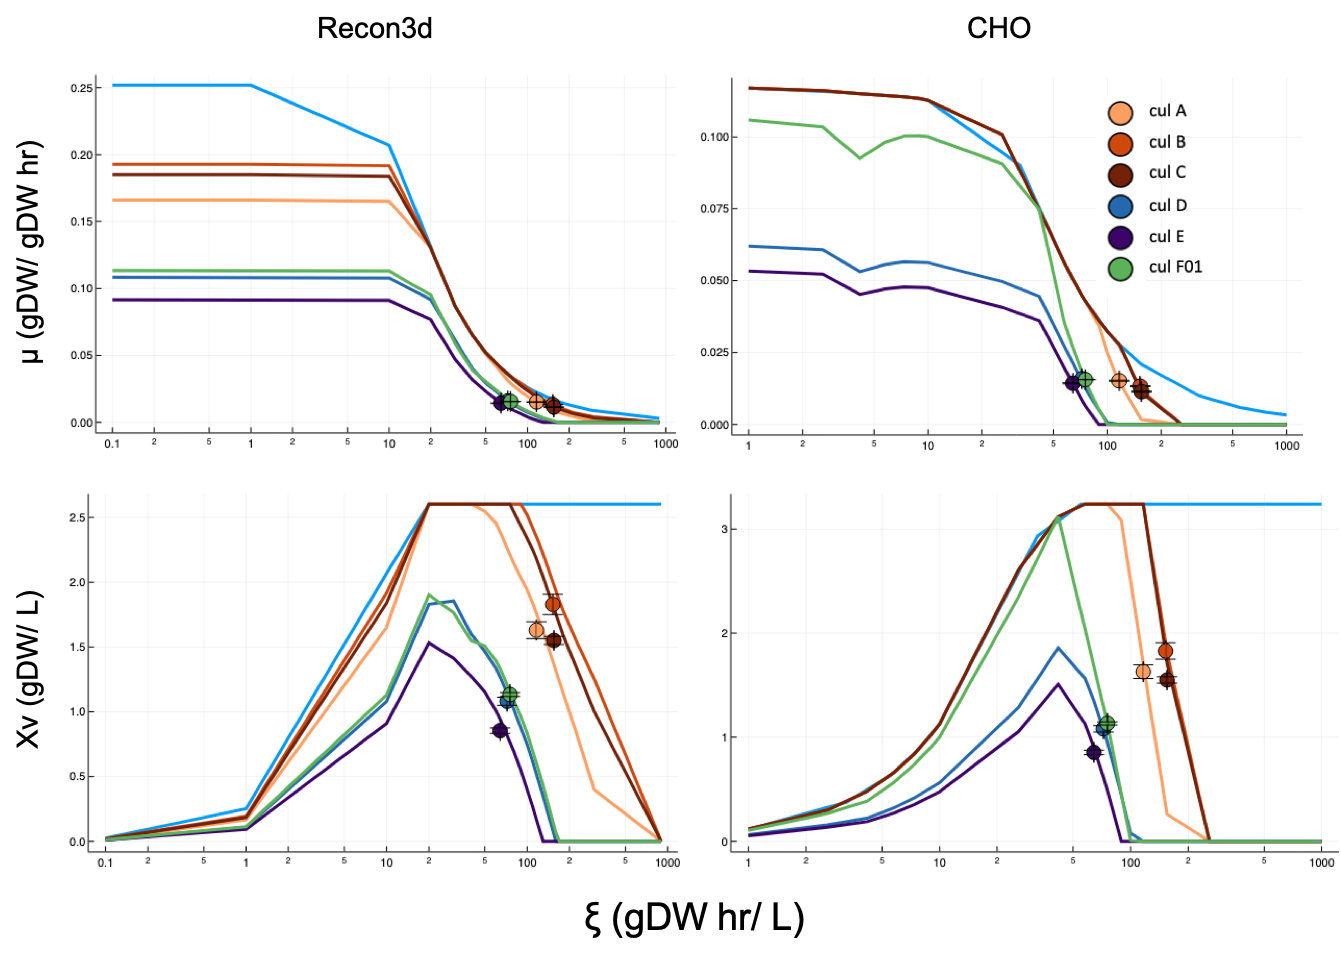
\includegraphics[scale = 0.5]{rich_medium_1}
		\caption{EP and FBA results showing the growth rate and the viable cell density dependence of $\xi$ for the six culture conditions. The solid lines represents the model predictions and the color points shows the experimental results. FBA results are shown as the solid light blue line.}
		
	\end{figure}

	\begin{figure}[h]
		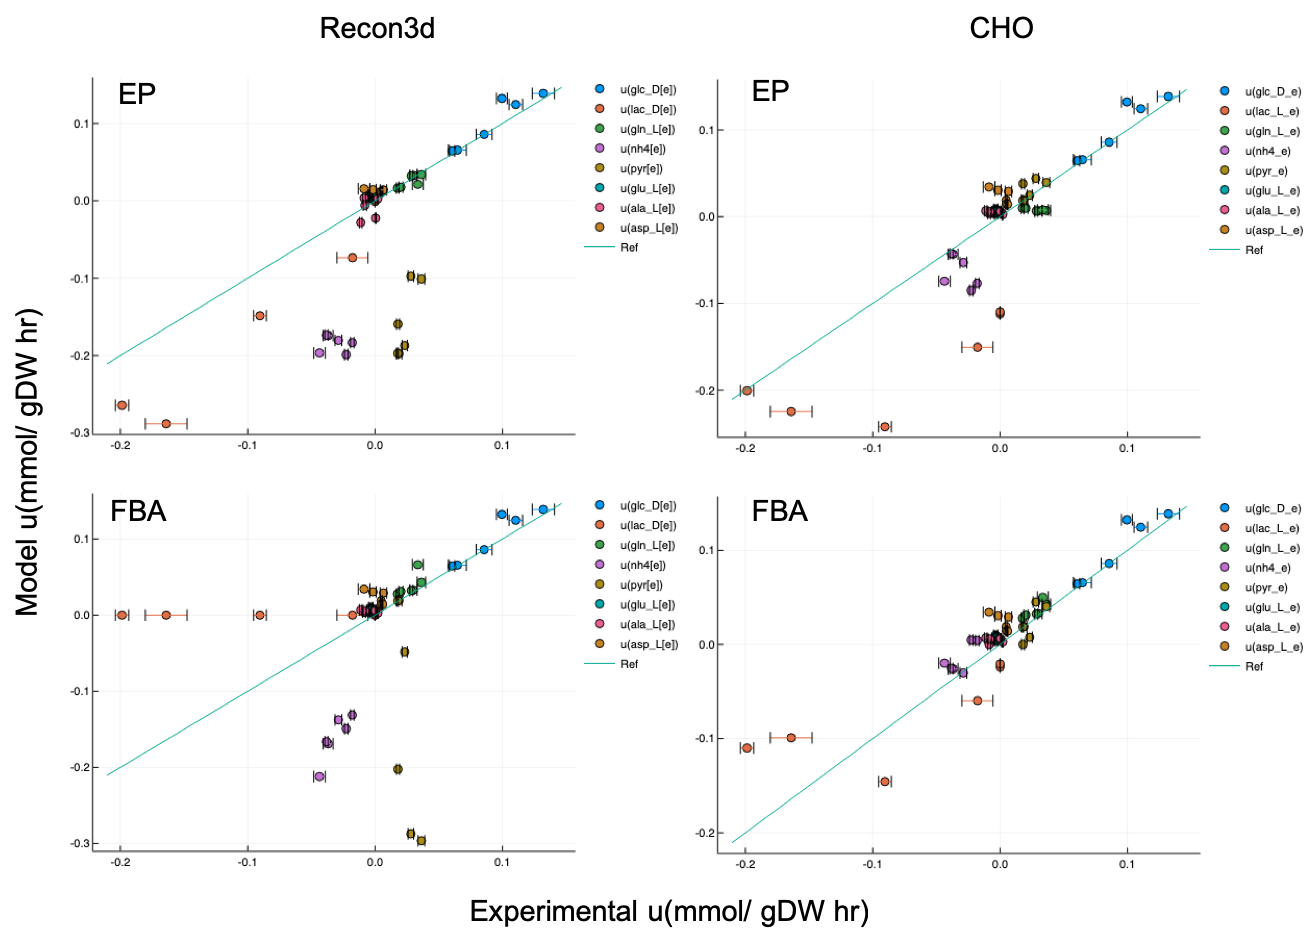
\includegraphics[scale = 0.5]{rich_medium_2}
		\caption{Correlations of all the experimental uptakes compared with the predicted value from EP and FBA.}
		
	\end{figure}
	
	\begin{figure}[h]
		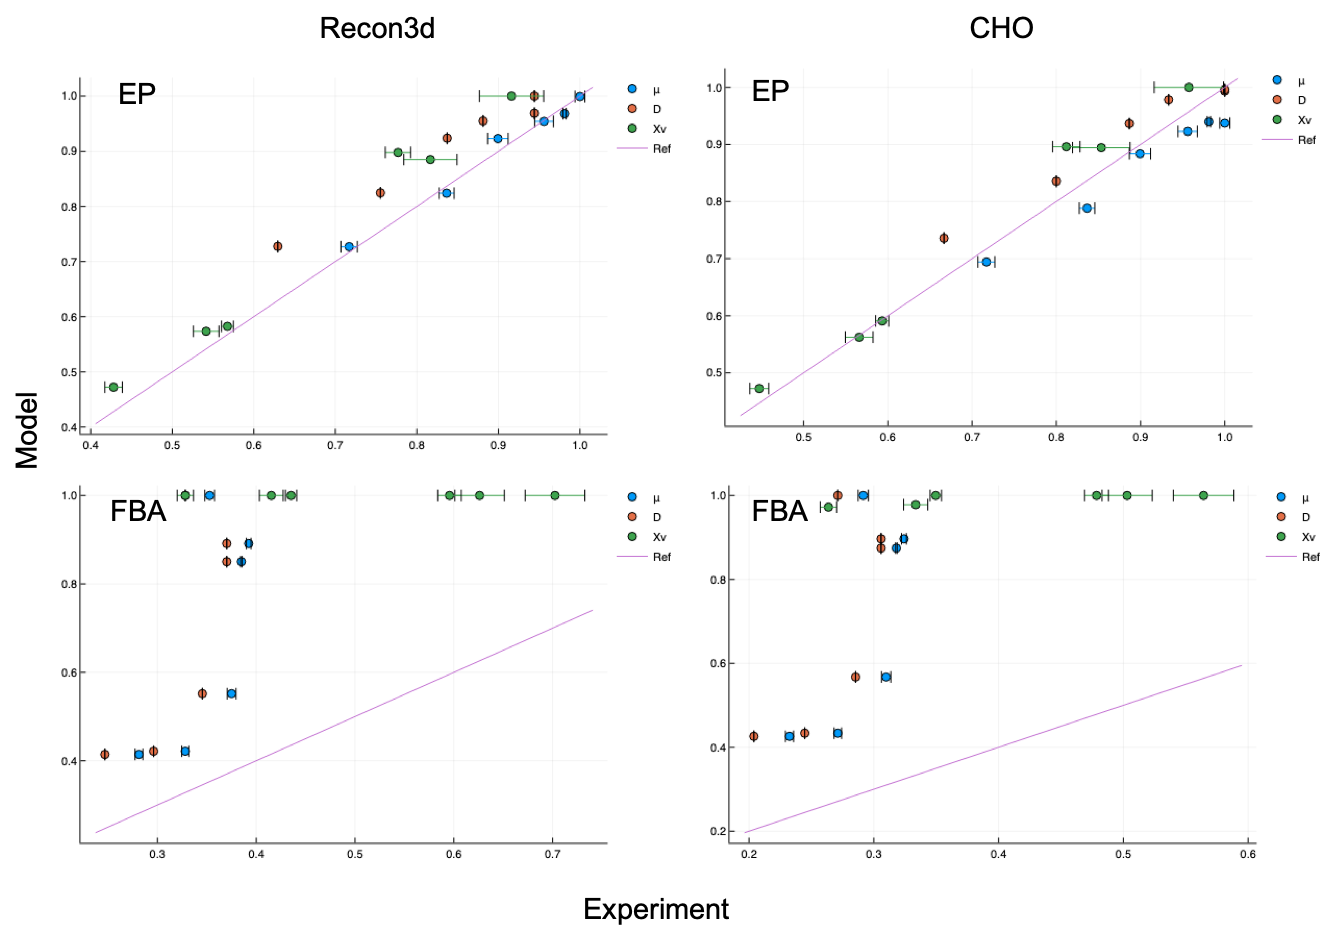
\includegraphics[scale = 0.5]{rich_medium_3}
		\caption{Normalized correlations of some experimental uptakes, growth rate, dilution rate and viable cell density compared with the predicted value from EP and FBA}
		
	\end{figure}

\section{Bibliography} %%%%%%%%%%%%%%%%%%%%%%%%%%%%%%%%%%%%%%%%%%%%%%%
		
\end{document}
